\documentclass{standalone}
\usepackage{tikz}
\usetikzlibrary{patterns, positioning}
\usepackage[sfdefault]{ClearSans} %% option 'sfdefault' activates Clear Sans as the default text font
\usepackage[T1]{fontenc}

\begin{document}
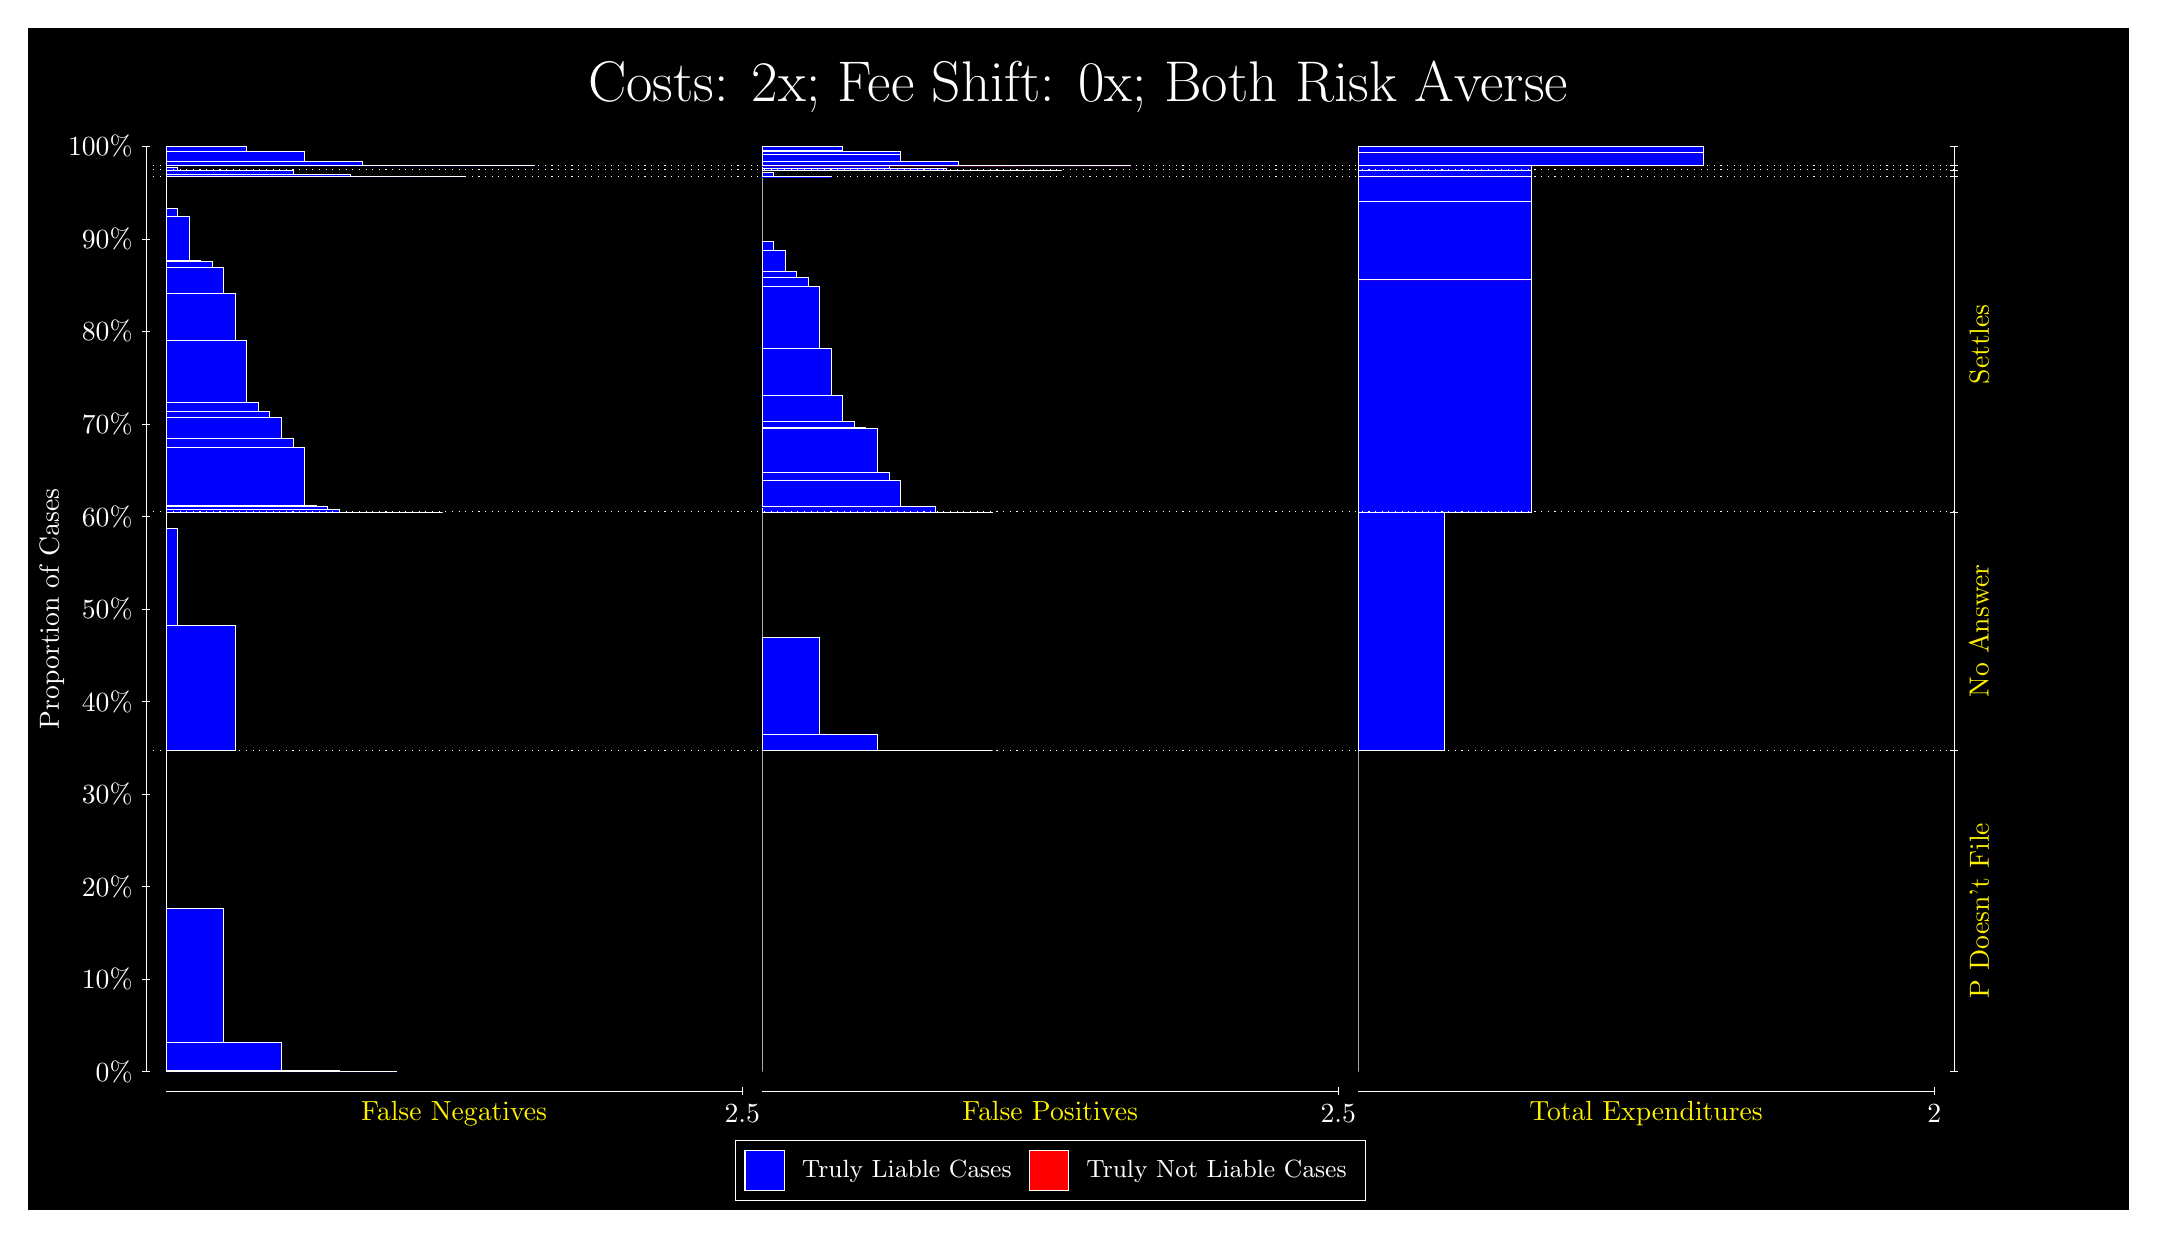
\begin{tikzpicture}
\draw[fill=black] (0,0) rectangle (26.667,15);
\draw[text=white] (0,13.5) rectangle (26.667,15) node[midway] {\huge Costs: 2x; Fee Shift: 0x; Both Risk Averse};
\draw[white, very thin] (1.5,1.75) -- (1.5,13.5);
\node[rotate=90, text=white, anchor=center] at (0.3, 7.625) {Proportion of Cases};
\draw[white, very thin] (1.45,1.75) -- (1.55,1.75);
\node[text=white, anchor=east] at (1.45, 1.75) {0\%};
\draw[white, very thin] (1.45,2.925) -- (1.55,2.925);
\node[text=white, anchor=east] at (1.45, 2.925) {10\%};
\draw[white, very thin] (1.45,4.1) -- (1.55,4.1);
\node[text=white, anchor=east] at (1.45, 4.1) {20\%};
\draw[white, very thin] (1.45,5.275) -- (1.55,5.275);
\node[text=white, anchor=east] at (1.45, 5.275) {30\%};
\draw[white, very thin] (1.45,6.45) -- (1.55,6.45);
\node[text=white, anchor=east] at (1.45, 6.45) {40\%};
\draw[white, very thin] (1.45,7.625) -- (1.55,7.625);
\node[text=white, anchor=east] at (1.45, 7.625) {50\%};
\draw[white, very thin] (1.45,8.8) -- (1.55,8.8);
\node[text=white, anchor=east] at (1.45, 8.8) {60\%};
\draw[white, very thin] (1.45,9.975) -- (1.55,9.975);
\node[text=white, anchor=east] at (1.45, 9.975) {70\%};
\draw[white, very thin] (1.45,11.15) -- (1.55,11.15);
\node[text=white, anchor=east] at (1.45, 11.15) {80\%};
\draw[white, very thin] (1.45,12.325) -- (1.55,12.325);
\node[text=white, anchor=east] at (1.45, 12.325) {90\%};
\draw[white, very thin] (1.45,13.5) -- (1.55,13.5);
\node[text=white, anchor=east] at (1.45, 13.5) {100\%};

\draw[white, very thin] (24.457,1.75) -- (24.457,13.5);
\draw[white, very thin] (24.407,1.75) -- (24.507,1.75);
\node[anchor=west] at (24.407, 1.75) {};
\draw[white, very thin] (24.407,5.8324) -- (24.507,5.8324);
\node[anchor=west] at (24.407, 5.8324) {};
\draw[white, very thin] (24.407,8.8572) -- (24.507,8.8572);
\node[anchor=west] at (24.407, 8.8572) {};
\draw[white, very thin] (24.407,13.115) -- (24.507,13.115);
\node[anchor=west] at (24.407, 13.115) {};
\draw[white, very thin] (24.407,13.2) -- (24.507,13.2);
\node[anchor=west] at (24.407, 13.2) {};
\draw[white, very thin] (24.407,13.254) -- (24.507,13.254);
\node[anchor=west] at (24.407, 13.254) {};
\draw[white, very thin] (24.407,13.5) -- (24.507,13.5);
\node[anchor=west] at (24.407, 13.5) {};

\draw[white, very thin, fill=blue] (1.75,1.75) rectangle (4.6775,1.7501);
\draw[white, very thin, fill=blue] (1.75,1.7501) rectangle (3.9457,1.7614);
\draw[white, very thin, fill=blue] (1.75,1.7614) rectangle (3.2138,2.1184);
\draw[white, very thin, fill=blue] (1.75,2.1184) rectangle (2.4819,3.8213);
\draw[white, very thin, fill=red] (1.75,3.8213) rectangle (1.75,3.8213);
\draw[white, very thin, fill=blue] (1.75,3.8213) rectangle (1.75,5.8324);
\draw[white, very thin, fill=blue] (1.75,5.8324) rectangle (2.6283,7.4212);
\draw[white, very thin, fill=blue] (1.75,7.4212) rectangle (1.8964,8.6535);
\draw[white, very thin, fill=red] (1.75,8.6535) rectangle (1.75,8.6535);
\draw[white, very thin, fill=blue] (1.75,8.6535) rectangle (1.75,8.8572);
\draw[white, very thin, fill=blue] (1.75,8.8572) rectangle (5.2631,8.8572);
\draw[white, very thin, fill=blue] (1.75,8.8572) rectangle (4.6775,8.8572);
\draw[white, very thin, fill=blue] (1.75,8.8572) rectangle (4.5312,8.8583);
\draw[white, very thin, fill=blue] (1.75,8.8583) rectangle (4.3848,8.8583);
\draw[white, very thin, fill=blue] (1.75,8.8583) rectangle (4.092,8.8586);
\draw[white, very thin, fill=blue] (1.75,8.8586) rectangle (3.9457,8.8911);
\draw[white, very thin, fill=blue] (1.75,8.8911) rectangle (3.7993,8.9301);
\draw[white, very thin, fill=blue] (1.75,8.9301) rectangle (3.6529,8.9357);
\draw[white, very thin, fill=blue] (1.75,8.9357) rectangle (3.5065,9.6801);
\draw[white, very thin, fill=blue] (1.75,9.6801) rectangle (3.3602,9.7891);
\draw[white, very thin, fill=blue] (1.75,9.7891) rectangle (3.2138,10.054);
\draw[white, very thin, fill=blue] (1.75,10.054) rectangle (3.0674,10.129);
\draw[white, very thin, fill=blue] (1.75,10.129) rectangle (3.0674,10.138);
\draw[white, very thin, fill=blue] (1.75,10.138) rectangle (2.921,10.254);
\draw[white, very thin, fill=blue] (1.75,10.254) rectangle (2.7746,11.043);
\draw[white, very thin, fill=blue] (1.75,11.043) rectangle (2.6283,11.63);
\draw[white, very thin, fill=blue] (1.75,11.63) rectangle (2.4819,11.959);
\draw[white, very thin, fill=blue] (1.75,11.959) rectangle (2.3355,12.037);
\draw[white, very thin, fill=blue] (1.75,12.037) rectangle (2.3355,12.037);
\draw[white, very thin, fill=blue] (1.75,12.037) rectangle (2.1891,12.058);
\draw[white, very thin, fill=blue] (1.75,12.058) rectangle (2.0428,12.61);
\draw[white, very thin, fill=blue] (1.75,12.61) rectangle (1.8964,12.711);
\draw[white, very thin, fill=red] (1.75,12.711) rectangle (1.75,12.711);
\draw[white, very thin, fill=blue] (1.75,12.711) rectangle (1.75,13.115);
\draw[white, very thin, fill=blue] (1.75,13.115) rectangle (5.5558,13.115);
\draw[white, very thin, fill=blue] (1.75,13.115) rectangle (4.8239,13.115);
\draw[white, very thin, fill=blue] (1.75,13.115) rectangle (4.092,13.147);
\draw[white, very thin, fill=blue] (1.75,13.147) rectangle (3.3602,13.199);
\draw[white, very thin, fill=blue] (1.75,13.199) rectangle (2.6283,13.2);
\draw[white, very thin, fill=red] (1.75,13.2) rectangle (1.75,13.2);
\draw[white, very thin, fill=blue] (1.75,13.2) rectangle (2.6283,13.201);
\draw[white, very thin, fill=blue] (1.75,13.201) rectangle (1.8964,13.234);
\draw[white, very thin, fill=red] (1.75,13.234) rectangle (1.75,13.234);
\draw[white, very thin, fill=blue] (1.75,13.234) rectangle (1.75,13.254);
\draw[white, very thin, fill=blue] (1.75,13.254) rectangle (6.4341,13.254);
\draw[white, very thin, fill=blue] (1.75,13.254) rectangle (5.7022,13.254);
\draw[white, very thin, fill=blue] (1.75,13.254) rectangle (4.9703,13.258);
\draw[white, very thin, fill=blue] (1.75,13.258) rectangle (4.2384,13.315);
\draw[white, very thin, fill=blue] (1.75,13.315) rectangle (3.5065,13.439);
\draw[white, very thin, fill=blue] (1.75,13.439) rectangle (2.7746,13.496);
\draw[white, very thin, fill=blue] (1.75,13.496) rectangle (2.0428,13.5);
\draw[white, very thin, fill=red] (1.75,13.5) rectangle (1.75,13.5);
\draw[white, very thin, fill=blue] (1.75,13.5) rectangle (1.75,13.5);
\draw[white, very thin, fill=red] (9.3189,1.75) rectangle (9.3189,1.75);
\draw[white, very thin, fill=blue] (9.3189,1.75) rectangle (9.3189,5.8324);
\draw[white, very thin, fill=red] (9.3189,5.8324) rectangle (12.246,5.8324);
\draw[white, very thin, fill=blue] (9.3189,5.8324) rectangle (12.246,5.8324);
\draw[white, very thin, fill=blue] (9.3189,5.8324) rectangle (11.515,5.8334);
\draw[white, very thin, fill=blue] (9.3189,5.8334) rectangle (10.783,6.0361);
\draw[white, very thin, fill=blue] (9.3189,6.0361) rectangle (10.051,7.2683);
\draw[white, very thin, fill=blue] (9.3189,7.2683) rectangle (9.3189,8.8572);
\draw[white, very thin, fill=red] (9.3189,8.8572) rectangle (12.246,8.8572);
\draw[white, very thin, fill=blue] (9.3189,8.8572) rectangle (12.246,8.8573);
\draw[white, very thin, fill=red] (9.3189,8.8573) rectangle (11.954,8.8573);
\draw[white, very thin, fill=blue] (9.3189,8.8573) rectangle (11.954,8.8573);
\draw[white, very thin, fill=red] (9.3189,8.8573) rectangle (11.661,8.8573);
\draw[white, very thin, fill=blue] (9.3189,8.8573) rectangle (11.661,8.8577);
\draw[white, very thin, fill=blue] (9.3189,8.8577) rectangle (11.515,8.9226);
\draw[white, very thin, fill=red] (9.3189,8.9226) rectangle (11.368,8.9226);
\draw[white, very thin, fill=blue] (9.3189,8.9226) rectangle (11.368,8.9228);
\draw[white, very thin, fill=blue] (9.3189,8.9228) rectangle (11.222,8.9256);
\draw[white, very thin, fill=red] (9.3189,8.9256) rectangle (11.075,8.9256);
\draw[white, very thin, fill=blue] (9.3189,8.9256) rectangle (11.075,9.2611);
\draw[white, very thin, fill=blue] (9.3189,9.2611) rectangle (10.929,9.3621);
\draw[white, very thin, fill=blue] (9.3189,9.3621) rectangle (10.783,9.9145);
\draw[white, very thin, fill=blue] (9.3189,9.9145) rectangle (10.636,9.9349);
\draw[white, very thin, fill=red] (9.3189,9.9349) rectangle (10.49,9.9349);
\draw[white, very thin, fill=blue] (9.3189,9.9349) rectangle (10.49,9.935);
\draw[white, very thin, fill=blue] (9.3189,9.935) rectangle (10.49,10.013);
\draw[white, very thin, fill=blue] (9.3189,10.013) rectangle (10.344,10.342);
\draw[white, very thin, fill=blue] (9.3189,10.342) rectangle (10.197,10.929);
\draw[white, very thin, fill=blue] (9.3189,10.929) rectangle (10.051,11.718);
\draw[white, very thin, fill=blue] (9.3189,11.718) rectangle (9.9044,11.835);
\draw[white, very thin, fill=blue] (9.3189,11.835) rectangle (9.758,11.843);
\draw[white, very thin, fill=blue] (9.3189,11.843) rectangle (9.758,11.918);
\draw[white, very thin, fill=blue] (9.3189,11.918) rectangle (9.6116,12.183);
\draw[white, very thin, fill=blue] (9.3189,12.183) rectangle (9.4652,12.292);
\draw[white, very thin, fill=blue] (9.3189,12.292) rectangle (9.3189,13.115);
\draw[white, very thin, fill=red] (9.3189,13.115) rectangle (10.197,13.115);
\draw[white, very thin, fill=blue] (9.3189,13.115) rectangle (10.197,13.116);
\draw[white, very thin, fill=blue] (9.3189,13.116) rectangle (9.4652,13.168);
\draw[white, very thin, fill=blue] (9.3189,13.168) rectangle (9.3189,13.2);
\draw[white, very thin, fill=red] (9.3189,13.2) rectangle (13.125,13.2);
\draw[white, very thin, fill=blue] (9.3189,13.2) rectangle (13.125,13.2);
\draw[white, very thin, fill=blue] (9.3189,13.2) rectangle (12.393,13.2);
\draw[white, very thin, fill=blue] (9.3189,13.2) rectangle (11.661,13.22);
\draw[white, very thin, fill=blue] (9.3189,13.22) rectangle (10.929,13.253);
\draw[white, very thin, fill=blue] (9.3189,13.253) rectangle (10.197,13.254);
\draw[white, very thin, fill=red] (9.3189,13.254) rectangle (14.003,13.254);
\draw[white, very thin, fill=blue] (9.3189,13.254) rectangle (14.003,13.254);
\draw[white, very thin, fill=red] (9.3189,13.254) rectangle (13.271,13.254);
\draw[white, very thin, fill=blue] (9.3189,13.254) rectangle (13.271,13.254);
\draw[white, very thin, fill=red] (9.3189,13.254) rectangle (12.539,13.254);
\draw[white, very thin, fill=blue] (9.3189,13.254) rectangle (12.539,13.258);
\draw[white, very thin, fill=blue] (9.3189,13.258) rectangle (11.807,13.315);
\draw[white, very thin, fill=red] (9.3189,13.315) rectangle (11.807,13.315);
\draw[white, very thin, fill=blue] (9.3189,13.315) rectangle (11.807,13.315);
\draw[white, very thin, fill=blue] (9.3189,13.315) rectangle (11.075,13.404);
\draw[white, very thin, fill=red] (9.3189,13.404) rectangle (11.075,13.404);
\draw[white, very thin, fill=blue] (9.3189,13.404) rectangle (11.075,13.439);
\draw[white, very thin, fill=blue] (9.3189,13.439) rectangle (10.344,13.454);
\draw[white, very thin, fill=blue] (9.3189,13.454) rectangle (10.344,13.496);
\draw[white, very thin, fill=blue] (9.3189,13.496) rectangle (9.6116,13.496);
\draw[white, very thin, fill=blue] (9.3189,13.496) rectangle (9.6116,13.5);
\draw[white, very thin, fill=blue] (9.3189,13.5) rectangle (9.3189,13.5);
\draw[white, very thin, fill=red] (16.888,1.75) rectangle (16.888,1.75);
\draw[white, very thin, fill=blue] (16.888,1.75) rectangle (16.888,5.8324);
\draw[white, very thin, fill=red] (16.888,5.8324) rectangle (17.986,5.8324);
\draw[white, very thin, fill=blue] (16.888,5.8324) rectangle (17.986,8.8572);
\draw[white, very thin, fill=red] (16.888,8.8572) rectangle (19.083,8.8572);
\draw[white, very thin, fill=blue] (16.888,8.8572) rectangle (19.083,11.806);
\draw[white, very thin, fill=red] (16.888,11.806) rectangle (19.083,11.806);
\draw[white, very thin, fill=blue] (16.888,11.806) rectangle (19.083,12.802);
\draw[white, very thin, fill=red] (16.888,12.802) rectangle (19.083,12.802);
\draw[white, very thin, fill=blue] (16.888,12.802) rectangle (19.083,13.115);
\draw[white, very thin, fill=red] (16.888,13.115) rectangle (19.083,13.115);
\draw[white, very thin, fill=blue] (16.888,13.115) rectangle (19.083,13.2);
\draw[white, very thin, fill=red] (16.888,13.2) rectangle (19.083,13.2);
\draw[white, very thin, fill=blue] (16.888,13.2) rectangle (19.083,13.254);
\draw[white, very thin, fill=red] (16.888,13.254) rectangle (21.279,13.254);
\draw[white, very thin, fill=blue] (16.888,13.254) rectangle (21.279,13.419);
\draw[white, very thin, fill=red] (16.888,13.419) rectangle (21.279,13.419);
\draw[white, very thin, fill=blue] (16.888,13.419) rectangle (21.279,13.5);
\draw[white, dotted] (1.5,5.8324) -- (24.457,5.8324);
\draw[white, dotted] (1.5,8.8572) -- (24.457,8.8572);
\draw[white, dotted] (1.5,13.115) -- (24.457,13.115);
\draw[white, dotted] (1.5,13.2) -- (24.457,13.2);
\draw[white, dotted] (1.5,13.254) -- (24.457,13.254);
\draw[white, very thin] (1.75,1.5) -- (9.0689,1.5);
\node[text=yellow, anchor=north] at (5.4094, 1.5) {False Negatives};
\draw[white, very thin] (9.0689,1.45) -- (9.0689,1.55);
\node[text=white, anchor=north] at (9.0689, 1.45) {2.5};

\draw[white, very thin] (9.3189,1.5) -- (16.638,1.5);
\node[text=yellow, anchor=north] at (12.978, 1.5) {False Positives};
\draw[white, very thin] (16.638,1.45) -- (16.638,1.55);
\node[text=white, anchor=north] at (16.638, 1.45) {2.5};

\draw[white, very thin] (16.888,1.5) -- (24.207,1.5);
\node[text=yellow, anchor=north] at (20.547, 1.5) {Total Expenditures};
\draw[white, very thin] (24.207,1.45) -- (24.207,1.55);
\node[text=white, anchor=north] at (24.207, 1.45) {2};

\node[text=yellow, centered, rotate=90] at (24.777, 3.7912) {P Doesn't File};
\node[text=yellow, centered, rotate=90] at (24.777, 7.3448) {No Answer};
\node[text=yellow, centered, rotate=90] at (24.777, 10.986) {Settles};




\draw (12.978300999999998,1.5) node[draw=none] (baseCoordinate) {};
\begin{scope}[align=center]
        \matrix[scale=0.5, draw=white, below=0.5cm of baseCoordinate, nodes={draw}, column sep=0.1cm]{
            \node[rectangle, draw, minimum width=0.5cm, minimum height=0.5cm, fill=blue] {}; &
            \node[draw=none, font=\small, text=white] (B) {Truly Liable Cases}; &
            \node[rectangle, draw, minimum width=0.5cm, minimum height=0.5cm, fill=red] {}; &
            \node[draw=none, font=\small, text=white] (B) {Truly Not Liable Cases}; \\
            };
\end{scope}

\end{tikzpicture}
\end{document}